% -*- TeX-master: "main"; fill-column: 72 -*-

\section{Examples}
\label{examples}

This section contains a variety of examples of SBML Level~3 Version~1
documents employing the Flux Balance Constraints package.

\subsection{\FBC syntax examples}

These examples are provided to highlight the \FBCPackage syntax.

\subsubsection{Example one}

As shown in \ref{fig:example1} the first example is a simple four reaction pathway that transforms metabolite \textit{IN} to \textit{OUT}. To begin with it is possible to compactly describe this network in terms of its reaction stoichiometry as shown in \ref{tble:ex1nmat}.
\begin{table}[h]
  \centering
    \begin{tabular}{c|cccc}
          & R1 & R2 & X1 & X2 \\ \hline
        A & 1 &  0 & -1 & -1 \\
        B & 0 & -1 &  1 &  1 \\
    \end{tabular}
  \caption{Example one stoichiometric matrix, \Nmat}
  \label{tble:ex1nmat}
\end{table}


For the purpose of this example we will assume that there is:
%
\begin{enumerate}
  \item a maximum limit (upper bound) of one on the flux through reaction \textit{R1} and
  \item the objective function is the maximization of flux through reaction \textit{R2}.
\end{enumerate}

 

\begin{figure}[h]
  \centering
  % Requires \usepackage{graphicx}
  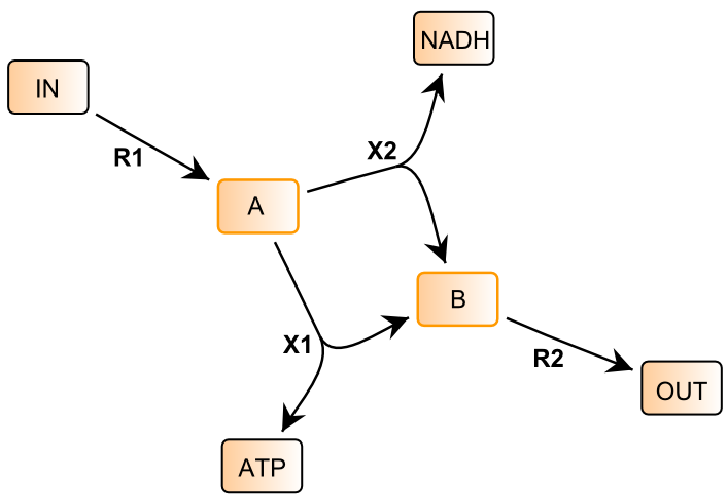
\includegraphics[width=8cm]{examples/spec-example1.pdf}\\
  \caption{\FBC syntax example: a simple four reaction pathway. The reactions are \textit{R1}, \textit{R2}, \textit{X1}, \textit{X2} with fixed species \textit{IN}, \textit{OUT}, \textit{ATP}, \textit{NADH} and variable species \textit{A}, \textit{B}.}
  \label{fig:example1}
\end{figure}




\exampleFile{examples/spec-example1.txt}
